% !TeX spellcheck = en_GB
\chapter{Literature Review}
\label{chp:LR}
As mentioned in Section \ref{sec:intro_bg}, \acl{cpp} is a subset of the general motion planning problem. This chapter will therefore begin with a brief overview of motion planning before discussing \acs{cpp} as a whole. Literature pertaining to \acs{cpp} is then discussed in several sections. Firstly, it is addressed in the context of the single robot \acs{cpp} problem. Several techniques used to achieve coverage using only one robot are summarized. 

Following this are three sections dedicated to the \acf{mcpp} problem. The first two cover distributed and non-distributed offline \acs{mcpp} respectively. This is followed by a section presenting some online \acs{mcpp} implementations. Many of the implementations were done with some application in mind, but the last section covers \acsp{uav} and how they have been applied to \acs{sar} operations in particular.

\section{Motion Planning}
\label{sec:LR-Motion Planning}
One of the most noteworthy items of literature presented on motion planning is by Lavalle \cite{Lavalle2006}. In this book, a differentiation is made between motion planning and trajectory planning. Motion planning, by their definition, refers to a series of translations and/or rotations required to get an agent from one point to another within some environment. Trajectory planning would then take this plan and find a strategy to execute it within the dynamic constraints of the agent. 

\emph{Agent} is a term from the field of artificial intelligence and is interchangeable with \emph{robot} or \emph{decision maker}. The agent will be what executes the plan once it is determined. Overall, a planning algorithm is used to develop a plan for the agent to execute within an environment. Execution generally refers to a real-world implementation of a plan on some device, for example, a \acs{uav}. It can also be performed in simulation. \cite{Lavalle2006}

The type of task that is executed as well as the environment it will be executed in are important for deciding on a motion planning algorithm.  The environment may be described as discrete or continuous. Some applications, such as solving a Rubik's cube, can be represented in a discrete manner \cite{Lavalle2006}. Most robotics applications, however, are in a continuous environment, which adds a layer of complexity to problem \cite{AIbook}.

Lavalle classifies motion planning problems into discrete and continuous. He discusses point-to-point path planning algorithms such as A* and Dijkstra's Algorithm in the context of discrete path planning. He then classifies continuous problems into two major categories, namely combinatorial and sampling-based methods.

The key difference between these methods is that combinatorial methods explicitly describe the environment, including obstacles, prior to searching and guarantee completeness. Sampling-based methods are generally resolution complete or probabilistically complete, which are more lax notions of completeness. Sampling-based methods sample points in the environment and tend to perform incremental collision avoidance during pathfinding. \cite{Lavalle2006}

The notion of completeness refers to the ability of a planning algorithm to correctly find a solution if one exists, otherwise reporting that there is no solution. Resolution completeness simply guarantees completeness only down to a certain resolution, and probabilistic completeness means that the probability of reporting a correct solution converges to one. \cite{Lavalle2006}

Sampling based methods are often better at dealing with a dynamic environment, whereas combinatorial methods, also known as exact methods, require exact knowledge of the environment beforehand and cannot handle dynamic obstacles without replanning, which is very inefficient. \acf{rrt} and \acf{prm} are respective examples of single and multi-query sampling-based methods. Combinatorial methods utilize methods like trapezoidal decompositions and Voronoi diagrams to generate roadmaps. Roadmaps in general can easily be navigated using discrete methods like A*. \cite{Lavalle2006}

Whenever developing a plan, the task could be to move from one point to another, change orientation, or to cover every point within an environment. The task could also involve multiple agents. Optimizing paths in these scenarios can be quite challenging because agents must now not only avoid collisions with obstacles in the environment, but also with one-another, while trying to achieve a certain goal. In the context of path planning with \acsp{uav}, the nature of the goal makes the problem fall into different categories, according to the authors of \cite{Zhang2020}. 

In a point-to-point problem, if the goal location is the same for all \acsp{uav}, it is referred to as a rendezvous task. If they all have different goal locations, it is an allocation task. And lastly, if the goal is not to move from a starting position to a goal, but instead to cover every point in an environment, it is called a coverage task. This classification is highlighted in Figure \ref{fig:MotionPlanning}.

One final concept to grasp for motion planning, is the difference between online and offline planners. Offline algorithms draw a distinct line between the planning phase and the execution phase. The entire plan is already developed prior to real-world (or simulation based) execution. Online planners tend to perform planning and execution in tandem. Generally, it senses the environment as it moves and computes the plan as it goes. The environment is not known a priori, as it is with offline planners. \cite{AIbook}
\begin{figure}[h!]
	\centering
	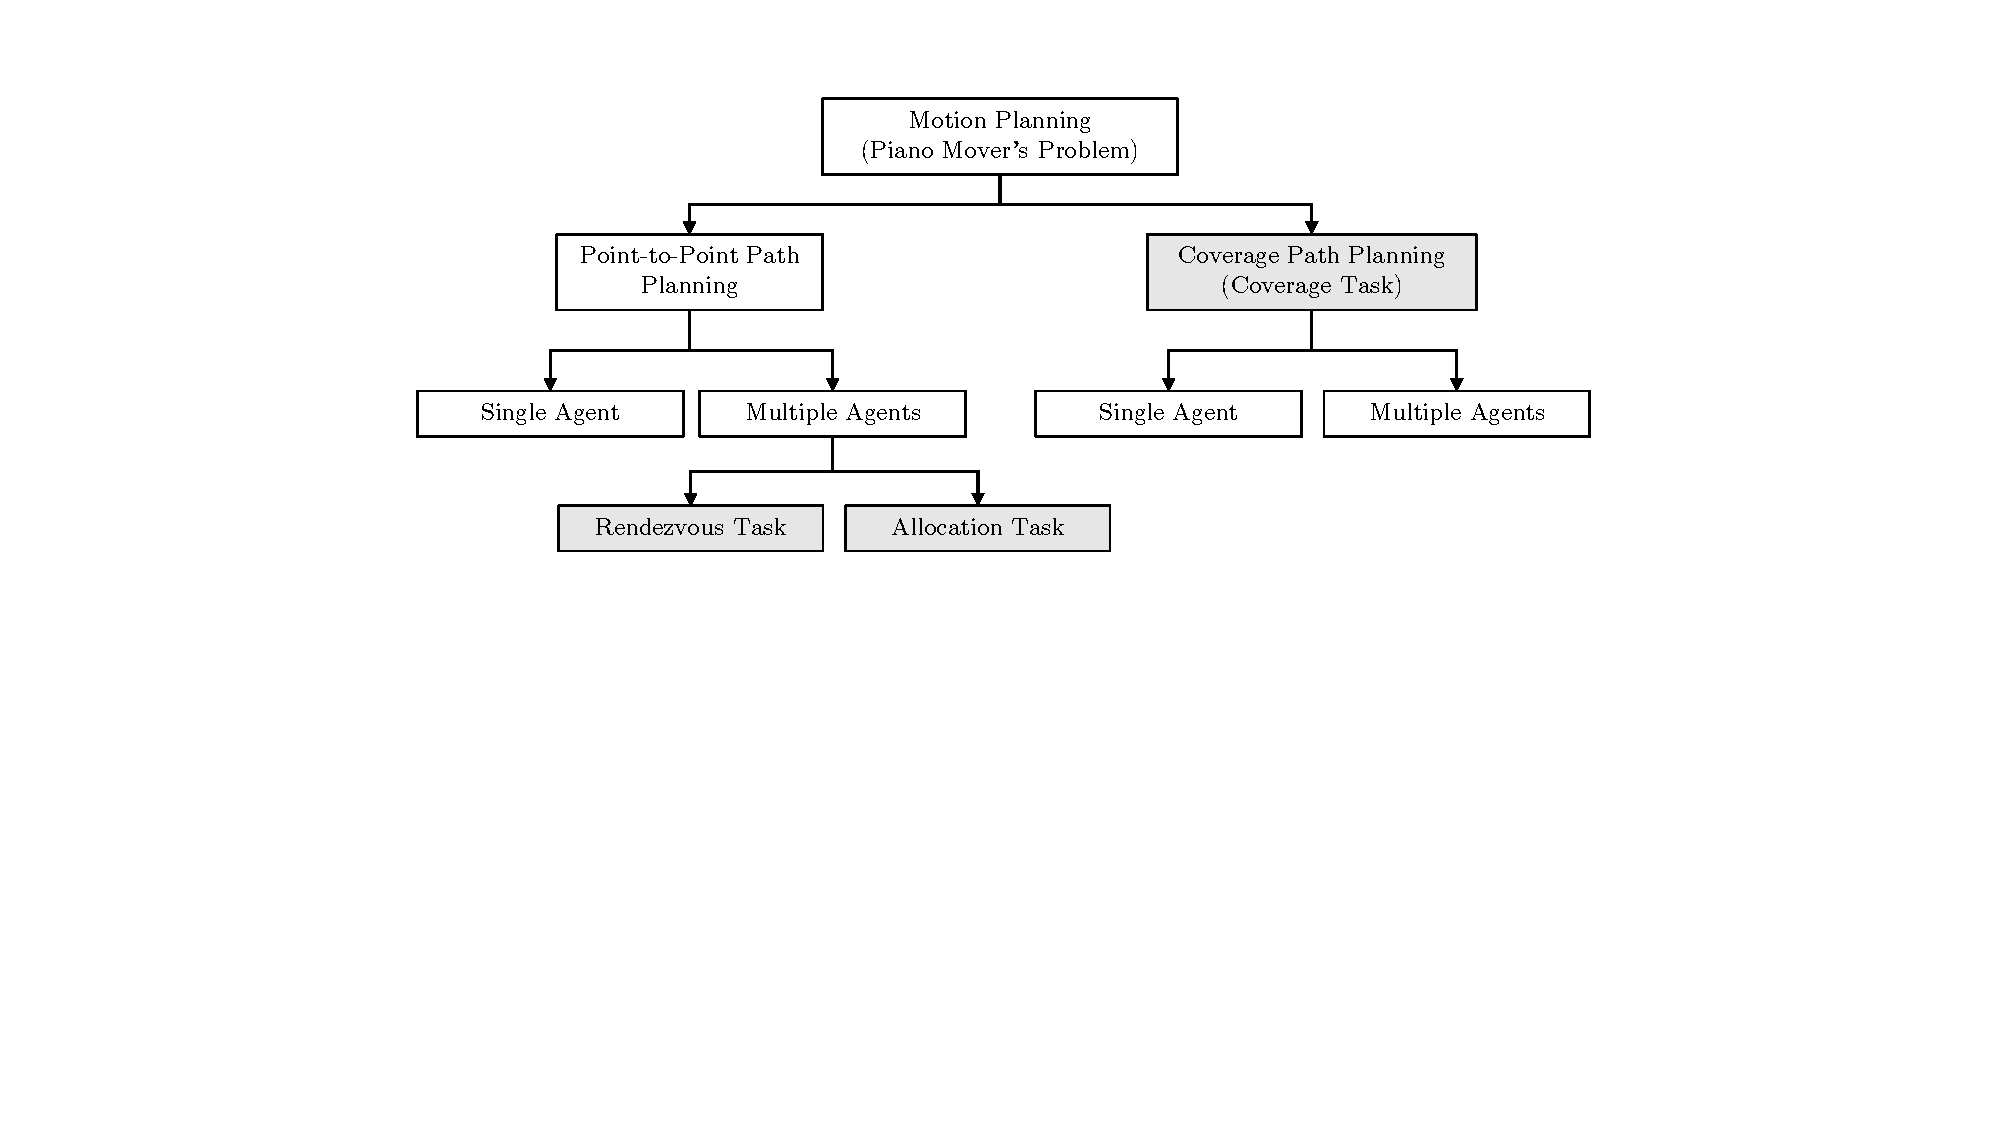
\includegraphics[width=\textwidth,trim={7cm 8.5cm 6.5cm 1.5cm},clip]{figs/Motion.pdf} % L  R
	\caption{Flow diagram showing a breakdown of the different kinds of path planning as part of motion planning.}
	\label{fig:MotionPlanning}
\end{figure}
\section{Coverage Path Planning}
\label{sec:LR-CPP}
% What is coverage path planning
\acf{cpp} is a subset of the general motion planning problem. The coverage task refers to visiting all points within an environment as opposed to the general start-goal type task \cite{Zhang2020}. \acs{cpp} can fall into the same categories as motion planning. It can be classified as discrete or continuous, online or offline, and as a single or multiple agent problem.

% 2001 Survey
A number of surveys have been done to give an overview of the literature available and progress made in the field of \acs{cpp}. A survey was done in 2001 wherein Choset divides \acs{cpp} into four categories \cite{Choset2001}. In later papers this is known as Choset's taxonomy, and is widely used to describe different types of \acs{cpp} algorithms.

Choset addresses heuristic and/or randomized approaches and also looks at three type of cellular decompositions, namely approximate, semi-approximate and exact. He continues in briefly addressing the multi robot scenario. The cellular decompositions all rely on simplifying the environment to achieve provably complete coverage. 

% TODO: STC is an approximate method. maybe reference the section that discusses that, along with other approximate methods
The approximate methods mean the environment is modelled as a set of cells with equal size and shape, generally a grid. These algorithms can achieve complete coverage of the discrete approximation of the environment, but don't guarantee complete coverage for the actual environment. Exact cellular decompositions divide the environment into polygons and cover these using simple motions e.g. back-and-forth manoeuvres. This can achieve complete coverage of the actual environment, hence the term \emph{exact}. This is further discussed in Section \ref{sec:lit SR CPP - Exact}. 

% 2013 and 2019 Survey
In 2013, a survey was done regarding \acs{cpp} in robotics \cite{CPP-Survey-2013}. It expands on Choset's taxonomy and gives more detail on recent developments in each category. This paper also addresses \acs{cpp} in three-dimensional scenarios, and briefly looks at \acs{cpp} where \acf{slam} is applied due to localization uncertainties. 
% TODO: make sure you write 2D an 3D the same everywhere e.g two-dimensional
Another recent survey was published in 2019, that once again builds on Choset's taxonomy \cite{CPP-Survey-2019}. They spend more time discussing simple manoeuvres and contrast them with more complex solutions.

% 2020 Survey - multiple robots
Generally multi-robot approaches add a layer of complexity to \acs{cpp}. The most notable challenge that arises is collision avoidance. Robots need to cooperate to achieve coverage while not only avoiding collisions with obstacles, but also with each other. In 2020, a paper was compiled that specifically deals with cooperative path planning \cite{Zhang2020}. It surveys path planning with multiple \acsp{uav} for the purpose of achieving many different goals, coverage being one of them.
%TODO: make sure you dont hyphenate cooperative anywhere

% TODO: Should you mention Centralized vs Decentralized (2020 paper looks at that in more detail)

% Description of offline vs online and mention that the next sections are offline, offline and online
In this chapter, a number of \acs{cpp} techniques are explored. Methods using a single robot for coverage are discussed in Section \ref{sec:lit SR CPP}. Sections \ref{sec:lit Ditributed MCPP} and \ref{sec:lit Non-Distributed MCPP} refer to offline methods of \acf{mcpp} and Section \ref{sec:lit Online MCPP} looks at online methods. The sections that discuss offline methods are categorised as distributed and non-distributed.

% Definition of distributed
Distributed, for the purpose of this paper, refers to methods where the paths of individual \acsp{uav} do not overlap. They are expected to fly in their own isolated sub-regions within an environment. In non-distributed methods,\acsp{uav} are free to cross paths. The area division step is not performed and so their paths are simply computed simultaneously, with knowledge of which cells have already been visited. \cite{Juan2018}

\section{Single Robot Coverage Path Planning}
\label{sec:lit SR CPP}
Single robot coverage is discussed in some detail here because several of the \acs{mcpp} problems make use of them. Distributed problems tend to divide an environment into sub-regions that can then be covered using single robot techniques. Several of the other methods simply use the single robot methods and scale them to multiple robot applications. %TODO: Subsection breakdown
% Mention simple maneouvres
\subsection{Exact Methods}
\label{sec:lit SR CPP - Exact}
Combinatorial methods, as described by Lavalle, are also referred to as exact methods \cite{Lavalle2006}. Exact methods for \acs{cpp} make use of the same geometric principles to divide an area into cells. However, instead of creating a roadmap, an adjacency graph is created and used to move between cells. Each cell is then individually covered, generally using simple manoeuvres \cite{CPP-Survey-2013}. 

Each cell in the decomposition is a node in the adjacency graph. An exhaustive walk is used to ascertain the sequence in which to visit these nodes to achieve coverage. Simple manoeuvres, such as back-and-forth motions, are then used to cover each cell individually. These algorithms are complete, so will completely cover the environment when possible. \cite{Choset-Bous1997}

A popular method, that is mentioned in Lavalle's book, is the trapezoidal decomposition. This method decomposes an environment into trapezoids (convex cells) based on the vertices of polygonal obstacles \cite{Lavalle2006}.

The trapezoidal and boustrophedon decomposition methods are applicable in two-dimensional coverage problems. They are offline approaches, since the environment must be known a priori, and only operate with polygonal obstacles. The boustrophedon method reduces the number of cells by only looking at vertices where a line can extend both upwards and downward from it. This reduces the final length of the coverage path and makes it more efficient. \cite{CPP-Survey-2013} 
% Some simplifications of the environment are probably made to make it polygonal. The lower poly it is, the more approximate the method can become. Still more accurate than grid based though.

A more versatile exact method, that uses Morse functions for the decomposition, is also available \cite{Choset-Morse2000}. 
\subsection{A* Path Coverage Path Planning}
\subsection{Spanning Tree Coverage Path Planning}
\label{sec:lit SR CPP - STC}

\subsection{Wavefront Planning}
\subsection{Artificial Intelligence Based Planning}
\section{Distributed Offline MCPP}
\label{sec:lit Ditributed MCPP}
A well established offline coverage path planning approach involves the divide areas technique. This partitions an area into regions for individual robots to cover. Each robot should then be able to cover its area using one of the individual area coverage techniques mentioned in Section \ref{sec:lit SR CPP}.
%TODO: Distributed vs Non-distributed - give the definition for the purpose of this paper
\subsection{Hexagonal Segmentation}
\label{subsec:Hex}
A notable distributed approach uses regular hexagons to segment the area of interest \cite{Azpurua2018}. This implementation is reminiscent of the exact methods often used for single robot coverage path planning mentioned in Section \ref{sec:lit SR CPP - Exact}. Exact methods generally divide an area into arbitrarily sized polygons called cells. The robot moves between these cells and covers them using simple motions. In the multi-robot scenario, the area is still divided into cells, but they need to be distributed between the robots evenly for searching. The ideal situation is to assign equal sized areas to each robot so that their path lengths are similar and they can complete their paths at roughly the same time.\\
Hexagonal cells make it easier to assign cells to robots, seen as they are all of the same size. Hexagons are clustered using the K-means algorithm to ensure a similar number of cells are assigned to each robot. The seeds are synonymous with the robots, therefore once the seed locations are finalized for even cell distribution, the robot initial positions are established. The robots cannot start from any random location, which can be undesirable. \\
The hexagons that are assigned to a given robot are contiguous and form a sub-region that is then covered using simple manoeuvres. Back and forth motions are generally quite popular. Static obstacles are considered in this implementation, but the smallest obstacle resolution is the size of a hexagon which may not be very representative of the environment. Figure \ref{fig:Hex}, taken directly from their paper, illustrates the back and forth manoeuvres used to cover the hexagonal partitions. Black hexagons represent no-fly zones and/or static obstacles. The dark red, green and blue regions represent the sub-regions as they are assigned to the respective robots for coverage.\\
\begin{figure}[h!]
	\centering
	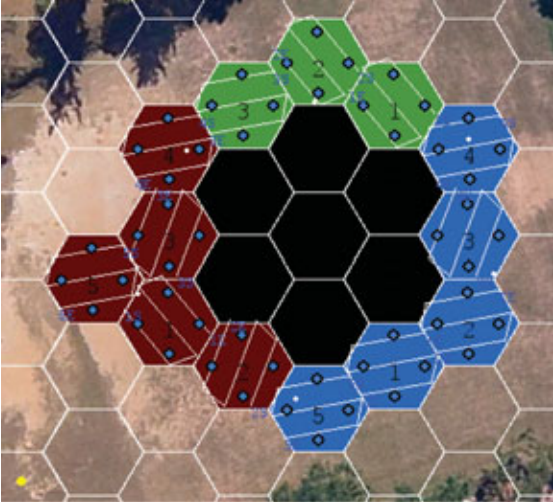
\includegraphics[scale=0.4]{figs/Hexagonal_Partitioning_Graphic}
	\caption{Simulation showing coverage of hexagonal partitions with back and forth motions with three robots. \cite{Azpurua2018}}
	\label{fig:Hex}
\end{figure}
\subsection{Voronoi Partitioning}
\label{subsec:Voronoi}
% Polygons
In the mathematics field, there are methods of area division to divide a polygon into a number of equal area polygons \cite{Nandakumar2012}. Another relevant method that also stems from the field of mathematics, is the Voronoi partition. This assigns regions within an area to seeds based on distance. The idea is that a region assigned to a seed represents all the points where the distance to that seed is shorter than to any other seed.\\
% Voronoi
% TODO: EDITING - Euclidean and Manhattan should always be with a capital letter 
If the Voronoi partition is applied to the \acs{mcpp} problem, the seeds become synonymous with robots. This partition works for any number of robots at any starting positions, but unless they are evenly spaced, the areas will not have equal sizes. Distances in these scenarios are usually Euclidean and the boundaries between areas represent the position where the distances from two seeds are equal.\\ 
The authors of \cite{Nair2020} implement \acs{mcpp} using Voronoi partitions in discrete space with static obstacles. They use square discretisation of the area and compare several different methods. They investigate geodesic-Manhattan-, Manhattan-, geodesic- and Euclidean-distance-based Voronoi partitions. \\
The Euclidean-based technique results in what the authors term "non-contiguous sub-regions". This means that cells that are part of a sub-region are not accessible by the robot assigned to them, due to obstacles within that sub-region. They solve this problem by using geodesic distance. This uses Euclidean measurements, but instead of a straight line distance between two cells, it calculates the distance using a collision free path between the two cells. \\
Another problem arises, due to their use of discrete space. This is that when using Euclidean distances, some cells were partially in two sub-regions instead of fully in one or the other. Their solution is to use Manhattan distances. Ultimately they claim to have solved these problems by using geodesic-Manhattan-based distances to generate the partition. And thus they coined the term \acf{gm}).\\
Figure \ref{fig:Voronoi} shows figures from the paper that show the results of an area division using different distance measures with a Voronoi partition.In both figures the black blocks represent obstacles, the round dots are the robot starting positions and the black lines over the grid represent the partition boundaries. \\
Figure \ref{fig:Voronoi - Euclid} shows the results using Euclidean distances. Here, the grey blocks are areas that would not be covered. This is clearly remedied using the GM-VPC technique in Figure \ref{fig:Voronoi - GM}. They implemented two different versions of \acs{gm}, which utilize respectively an exact and an approximate individual area search technique. They implemented a boustrophedon coverage plan for the exact solution and a spanning tree for the approximate version. Both of these performed better when using geodesic-Manhattan distances.   
\begin{figure}[h!]
	\centering
	\begin{subfigure}[b]{0.45\textwidth}
		\centering
		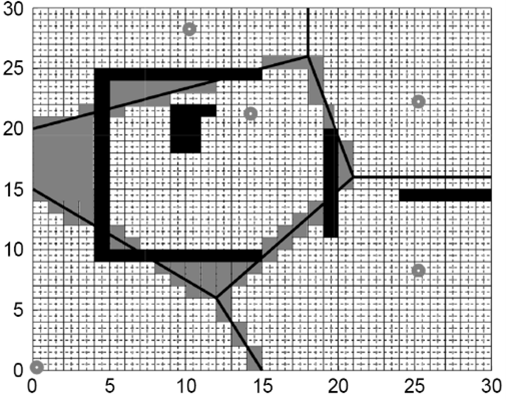
\includegraphics[scale=0.4]{figs/GM_VPC_Euclid}
		\caption{Euclidean}
		\label{fig:Voronoi - Euclid}
	\end{subfigure}
	\hfill
	\begin{subfigure}[b]{0.45\textwidth}
		\centering
		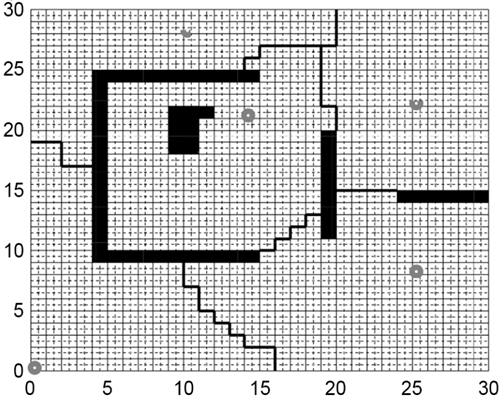
\includegraphics[scale=0.4]{figs/GM_VPC}
		\caption{Geodesic-Manhattan}
		\label{fig:Voronoi - GM}
	\end{subfigure}
\caption{Figures showing results for the Voronoi partitioning scheme for two different distance measures. \cite{Nair2020}}
\label{fig:Voronoi}
\end{figure}
\subsection{Negotiation Protocol}
\label{subsec:Negotiation}
A negotiation or bargaining protocol refers to a process involving task partitioning. In the context of area division for \acs{cpp}, the task represents the area to be divided \cite{Rossi2009}. The authors of \cite{Rossi2009} present a negotiation model based on Rubinstein's alternate-offers protocol, for the purpose of area division. The focus of their implementation was to develop a distributed algorithm capable of considering robot capabilities. This means that the robots wouldn't have to be homogeneous and can have different flight-time capabilities, manoeuvrability, on-board equipment and so forth \cite{Barrientos2011}.\\ 
They implemented their algorithm and found that it can achieve near optimum results. It tries to maximise the size of each robot's subdivision of the area (based on its capabilities), while also minimising sub-area overlap. The algorithm also works to avoid static obstacles or no fly zones that are present in the area. Moreover, they proved that it could be applied in a situation where re-planning may be necessary.\\
% Re-planning is necessary in a scenario when carrying out the plan changes the environment, thereby requireing replanning wiht the new environment scenario
% TODO: Future work - as new information about target becomes available - replan
A more complete implementation of the algorithm including an individual area search technique was also developed and tested \cite{Barrientos2011}. In this implementation they use a wavefront planner for the individual area coverage path generation. This requires discretisation of the area into cells. In their case, they used rectangles whose size was determined by on-board camera \acf{fov}. In order for the polygons generated by the negotiation protocol to work effectively, they use a method called Bresenham's line algorithm to approximate the lines that divide the areas in discrete space, so that they pass through the centroids of cells.\\
The area division achieved sometimes produces non-convex shapes, which the wavefront planner can handle effectively. Their implementation also minimizes energy consumption by minimizing the number of turns and not allowing backtracking. They also have the ability to specify the initial take-off positions of the robots. Distance from the specified take-off point to the starting point for sub-area coverage are considered in the sub-task negotiations. The authors also mention being able to specify robot landing positions pre-emptively.\\
One visible drawback in their implementation is that they coverage appears incomplete. The boundaries between areas pass through waypoints (cell centroids), that effectively get excluded from the coverage algorithm and are not covered. Using an exact method to search the individual areas could produce better results. Changing the boundaries to lie on the edges of cells rather than passing through their centroids could also make a difference.
\begin{figure}[h!]
	\centering
	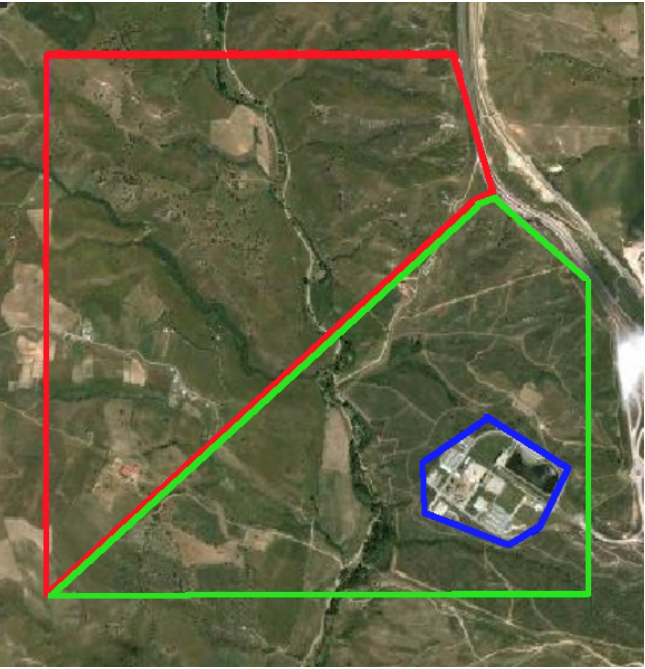
\includegraphics[scale=0.35]{figs/Negotiation_Protocol}
	\caption{Figure showing the resulting area partition using the negotiation protocol. This example is for two robots and includes a no fly zone. \cite{Rossi2009}}
	\label{fig:NegProt}
\end{figure}
\subsection{MSTC}
\label{subsec:mstc}
\acf{mstc} is a variant of single robot \acf{stc} as presented in Section \ref{sec:lit SR CPP - STC}. The authors of \cite{Hazon2005} designed the first variants of \acs{mstc}. The two variations they suggest are one that allows for backtracking and one that does not. Both variations still utilize a single spanning tree, but simply circumnavigate the tree with multiple robots instead of a single one.\\
They place a lot of emphasis on robustness and efficiency, in addition to completeness. They demonstrate an algorithm that segments the path around a spanning tree to evenly distribute it among robots. This distribution of robots is however, unrealistic. Their method becomes incredibly inefficient when robots are clustered closely together. This is because a robot simply navigates the path until it reaches the initial position of the next robot on the path.\\
Figure \ref{fig:MSTC} shows the paths that are generated when the robots are evenly distributed along the path that circumnavigates the tree. Blue dots represent the robot initial positions and the spanning tree is shown in red. The second method they suggest remedies this somewhat. It allows for backtracking and improves the efficiency.\\
The ideal situation is that all the robots have near equal path lengths, provided they are homogeneous robots. This is not guaranteed with this algorithm when the robots have random starting positions, but allowing for backtracking can improve the results and allow the coverage to be completed in a shorter amount of time.\\
\begin{figure}[h!]
	\centering
	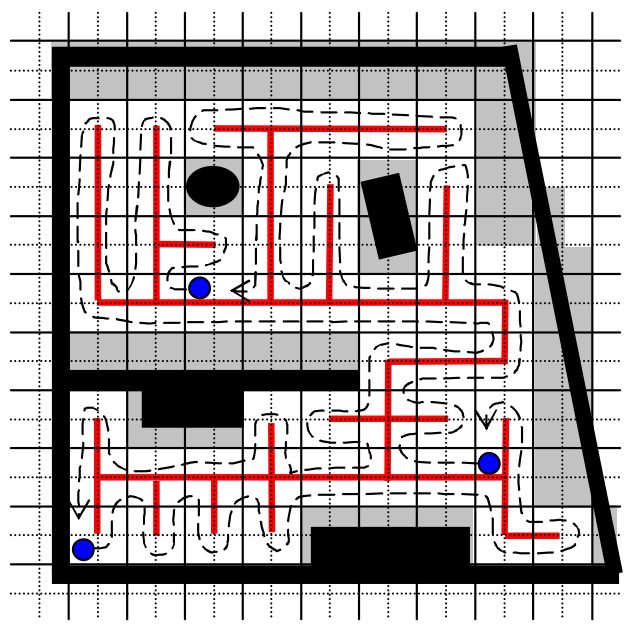
\includegraphics[scale=0.4]{figs/MSTC-Graphic}
	\caption{MSTC algorithm showing the paths for three robots on an environment grid. \cite{Hazon2005}}
	\label{fig:MSTC}
\end{figure}

\subsection{DARP}
\label{subsec:lit DARP}
\section{Non-Distributed Offline MCPP}
\label{sec:lit Non-Distributed MCPP}
\subsection{MFC}
% insert MFC
\acf{mfc} is a method that was developed by the authors in \cite{Zheng2005} to improve upon the \acs{mstc} method mentioned in Section \ref{subsec:mstc}. Their intent was to construct a tree with the consideration that it will be divided afterwards, unlike what \acs{mstc} does. It allows for robot path overlap, which means there is redundant coverage and collision avoidance would need to be considered. However it can handle unique scenarios, where backtracking is unavoidable, quite well.\\ 
Their implementation is based on an algorithm presented in \cite{Even2003}. This is an approximation algorithm and they specifically looked at the rooted tree cover scenario. The roots represent the robot initial positions and then a tree is generated for each robot, using the objective to minimize the weight of the maximum weight tree. These trees are each circumnavigated by their robot (root) to cover the area.\\
Based on the simulations they ran with \acs{mstc} and \acs{mfc}, they found that \acs{mfc} generated closer to optimum results and generally achieved coverage in a shorter amount of time.	Because there is path overlap in certain scenarios, \acs{mfc} is not a truly distributed method.
\subsection{Sampling-Based}
% Check Lavalle
\subsection{Artificial-Intelligence-Based}

%%%%%%%%%%%%%%%%%%%%%%%%%%%%%%%%%%%%%%%%%%%%%%%%%%%%%%%%%%%%%%%%%%%%%%%
\section{Online MCPP}
\label{sec:lit Online MCPP}
\section{UAVs and Search and Rescue}
%DroneSAR
%Rotary Wing vs Fixed-Wing UAVs}


